%%% Template para Relatório Técnico - UTFPR
%%% Baseado no template de Willian Chamma / Mikhail Klassen

\documentclass[12pt,a4paper, brazil]{article}

%%%%%%% INFORMAÇÕES DO CABEÇALHO
\newcommand{\workingDate}{\textsc{\selectlanguage{portuguese}\today}}
\newcommand{\userName}{LRCO7A}
\newcommand{\institution}{UTFPR-AP}
\usepackage{researchdiary_png}

\usepackage{listings}
\usepackage{float}
\usepackage{placeins}

% Configuração para código VHDL
\lstdefinestyle{vhdl}{
    language=VHDL,
    basicstyle=\ttfamily\small,
    keywordstyle=\color{blue}\bfseries,
    commentstyle=\color{gray}\itshape,
    stringstyle=\color{red},
    numbers=left,
    numberstyle=\tiny\color{gray},
    numbersep=5pt,
    frame=single,
    breaklines=true,
    captionpos=b,
    tabsize=2
}

\begin{document}

\begin{center}
{\textbf {\huge Atividade Prática 1 -- Portas Lógicas}}\\[5mm]
{\large Pedro Lucas dos Reis Silva - RA: 2272040} \\[5mm]
27/03/2026\\[5mm]
\end{center}

% ============================================================
\section{Introdução}
% ============================================================

Circuitos digitais combinacionais são aqueles cuja saída depende exclusivamente dos valores atuais das entradas, sem qualquer elemento de memória. As portas lógicas são os blocos fundamentais de construção desses circuitos, implementando as operações básicas da álgebra booleana.

Nesta atividade foram implementadas as seguintes portas lógicas em VHDL, com duas entradas (\texttt{a} e \texttt{b}) e uma saída independente para cada operação:

\begin{itemize}
    \item \textbf{NOT} (inversora) -- aplicada individualmente a cada entrada (z1 = NOT a, z2 = NOT b)
    \item \textbf{AND} -- saída 1 somente quando ambas as entradas são 1
    \item \textbf{OR} -- saída 1 quando pelo menos uma entrada é 1
    \item \textbf{NAND} -- inverso do AND
    \item \textbf{NOR} -- inverso do OR
    \item \textbf{XOR} -- saída 1 quando as entradas são diferentes
    \item \textbf{XNOR} -- saída 1 quando as entradas são iguais
\end{itemize}

\subsection{Conceitos VHDL}

A descrição em VHDL é composta por duas partes principais:

\begin{itemize}
    \item \textbf{Entity}: define a interface externa do circuito (portas de entrada e saída), equivalente ao símbolo de um componente num esquemático.
    \item \textbf{Architecture}: define o comportamento interno do circuito. Nesta atividade foi utilizada a descrição no estilo \textit{fluxo de dados} (dataflow), onde cada saída é descrita diretamente por sua equação booleana.
\end{itemize}

Todas as atribuições de sinal dentro da arquitetura (\texttt{<=}) executam em \textbf{paralelo}, refletindo o comportamento real do hardware: todas as portas operam simultaneamente. O tipo \texttt{bit} foi utilizado por aceitar apenas \texttt{'0'} ou \texttt{'1'}, suficiente para representar lógica digital básica.

Os códigos VHDL completos do circuito principal e do testbench encontram-se nos Apêndices \ref{ap:codigo-principal} e \ref{ap:testbench}, respectivamente.

% ============================================================
\section{Tabela Verdade}
% ============================================================

A Tabela \ref{tab:verdade} apresenta os resultados esperados para cada combinação de entrada, cobrindo todas as 8 operações lógicas implementadas.

\begin{table}[H]
\centering
\caption{Tabela verdade completa das 8 portas lógicas.}
\label{tab:verdade}
\begin{tabular}{@{}cc|cccccccc@{}}
\toprule
\textbf{a} & \textbf{b} & \textbf{z1} & \textbf{z2} & \textbf{z3} & \textbf{z4} & \textbf{z5} & \textbf{z6} & \textbf{z7} & \textbf{z8} \\
           &            & NOT a & NOT b & AND & OR & NAND & NOR & XOR & XNOR \\
\midrule
0 & 0 & 1 & 1 & 0 & 0 & 1 & 1 & 0 & 1 \\
0 & 1 & 1 & 0 & 0 & 1 & 1 & 0 & 1 & 0 \\
1 & 0 & 0 & 1 & 0 & 1 & 1 & 0 & 1 & 0 \\
1 & 1 & 0 & 0 & 1 & 1 & 0 & 0 & 0 & 1 \\
\bottomrule
\end{tabular}
\end{table}
\FloatBarrier

% ============================================================
\section{Simulação}
% ============================================================

A simulação foi realizada utilizando o GHDL (compilador e simulador VHDL open source) em ambiente Linux. O GHDL compilou o código VHDL, elaborou o circuito e executou a simulação gerando um arquivo de formas de onda no formato VCD (\textit{Value Change Dump}). A visualização dos sinais foi feita com o GTKWave.

O testbench aplica as 4 combinações possíveis de \texttt{a} e \texttt{b} (00, 01, 10, 11), cada uma com duração de 1 ns. A Figura \ref{fig:simulacao} apresenta as formas de onda obtidas, onde é possível verificar que os valores de cada saída correspondem exatamente à tabela verdade:

\begin{itemize}
    \item \textbf{z1 e z2 (NOT)}: são o inverso de \texttt{a} e \texttt{b}, respectivamente.
    \item \textbf{z3 (AND)}: só vai para 1 quando a=1 e b=1 (instante 3 ns).
    \item \textbf{z4 (OR)}: vai para 1 sempre que ao menos uma entrada é 1.
    \item \textbf{z5 e z6 (NAND e NOR)}: são exatamente o complemento de z3 e z4.
    \item \textbf{z7 (XOR)}: 1 quando as entradas diferem (instantes 1 e 2 ns).
    \item \textbf{z8 (XNOR)}: complemento do XOR, 1 quando as entradas são iguais.
\end{itemize}

\begin{figure}[H]
    \centering
    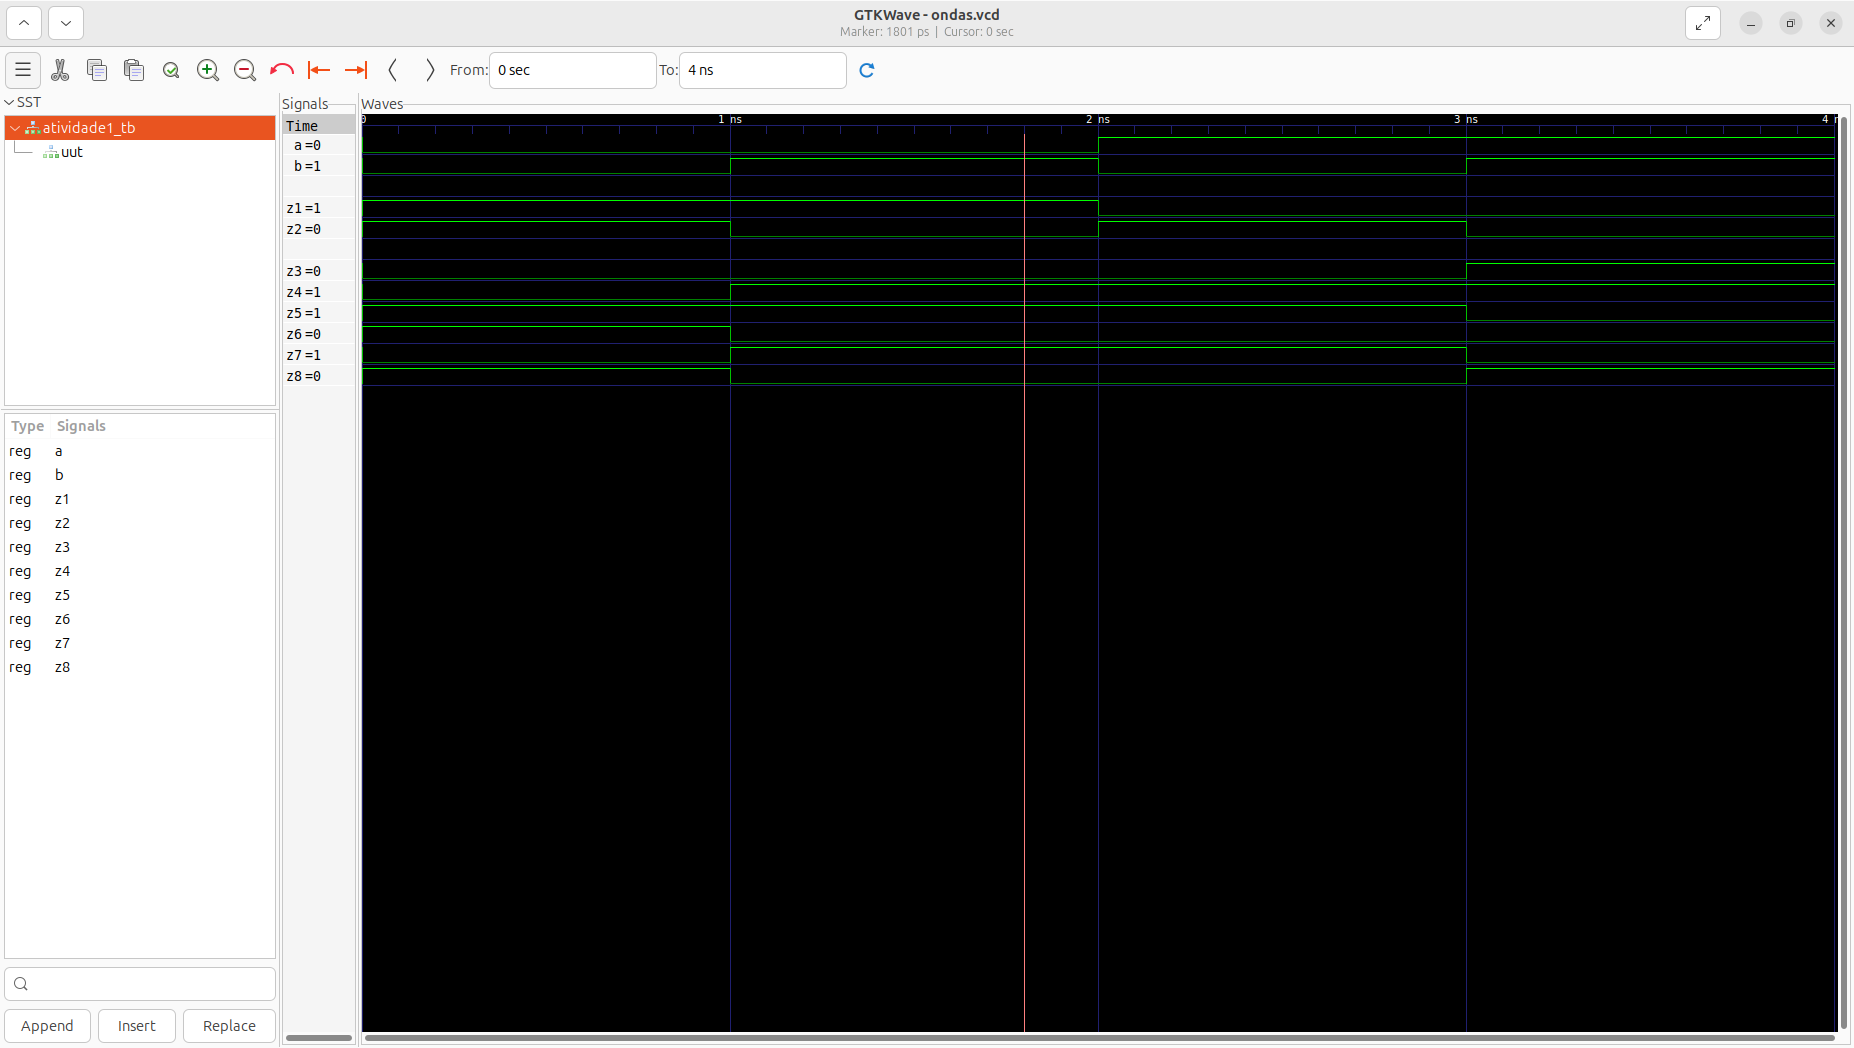
\includegraphics[width=0.95\textwidth]{simulacao1.png}
    \caption{Formas de onda da simulação das 8 portas lógicas, visualizadas no GTKWave.}
    \label{fig:simulacao}
\end{figure}
\FloatBarrier

% ============================================================
\section{Diagrama RTL}
% ============================================================

O diagrama RTL (\textit{Register Transfer Level}) representa a estrutura do circuito sintetizado, mostrando os componentes lógicos e suas interconexões. O código VHDL foi inserido no Quartus Prime e o diagrama foi gerado através da ferramenta \textit{RTL Viewer} (Tools $\rightarrow$ Netlist Viewers $\rightarrow$ RTL Viewer).

A Figura \ref{fig:rtl} apresenta o diagrama obtido, onde se observa que:

\begin{itemize}
    \item As entradas \texttt{a} e \texttt{b} alimentam diretamente todas as portas lógicas.
    \item Cada saída (z1 a z8) está conectada à sua respectiva porta lógica.
    \item O diagrama evidencia a natureza puramente combinacional do circuito, sem elementos de memória.
\end{itemize}

\begin{figure}[H]
    \centering
    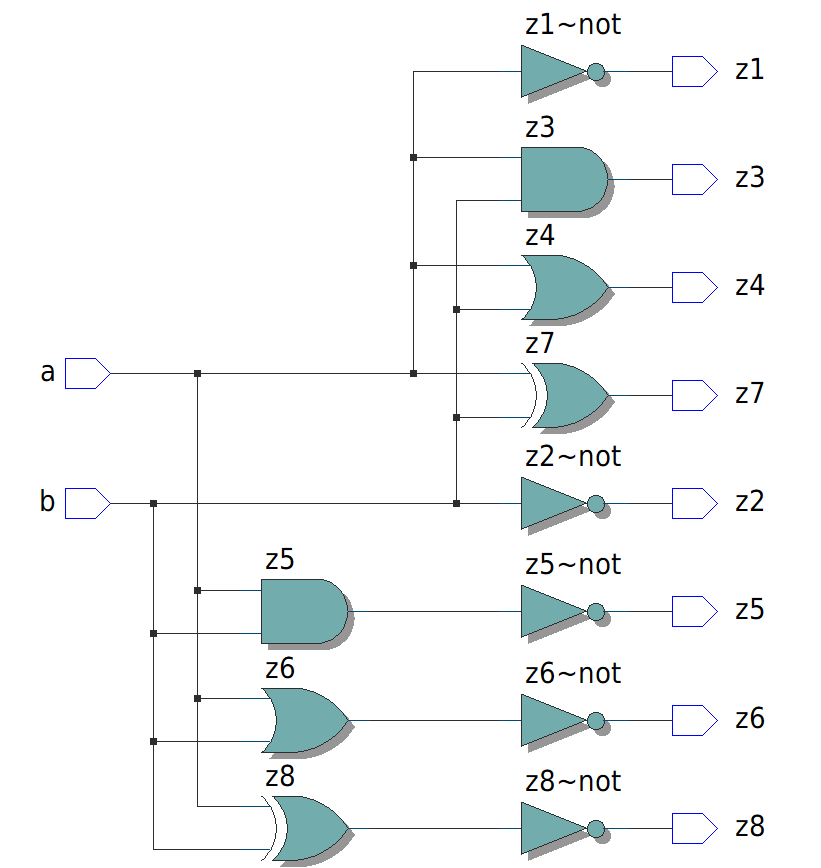
\includegraphics[width=0.95\textwidth]{rtl.png}
    \caption{Diagrama RTL do circuito, gerado pelo Quartus Prime (RTL Viewer).}
    \label{fig:rtl}
\end{figure}
\FloatBarrier

% ============================================================
\section{Ferramentas Utilizadas}
% ============================================================

O desenvolvimento desta atividade envolveu a utilização de diferentes ferramentas ao longo do processo:

\begin{itemize}
    \item \textbf{GHDL} (v4.1.0) -- compilador e simulador VHDL open source, utilizado para compilar o código e gerar as formas de onda em formato VCD.
    \item \textbf{GTKWave} (v3.3.116) -- visualizador de formas de onda open source, utilizado para analisar os sinais da simulação.
    \item \textbf{Quartus Prime Lite} -- ferramenta da Intel para síntese de circuitos em FPGA, utilizada para gerar o diagrama RTL do circuito.
    \item \textbf{VS Code} -- editor de texto com extensão VHDL para syntax highlighting.
\end{itemize}

Durante o desenvolvimento, foram testadas alternativas open source para a geração do diagrama RTL, como o Yosys (sintetizador RTL) e o Logisim (simulador de circuitos digitais). O Yosys conseguiu gerar o diagrama a partir de uma descrição equivalente em Verilog, porém a visualização resultante não ficou tão intuitiva quanto a do Quartus. O Logisim permitiu desenhar o circuito manualmente com os símbolos das portas, mas não realiza síntese a partir de VHDL.

Concluiu-se que, em princípio, é possível realizar todo o fluxo de simulação e visualização utilizando exclusivamente ferramentas open source (GHDL + GTKWave + Yosys), reservando o Quartus apenas para a etapa final de síntese e gravação na placa FPGA. No entanto, essa abordagem requer um estudo mais aprofundado da integração entre as ferramentas, em especial o plugin \texttt{ghdl-yosys} para leitura direta de VHDL no sintetizador.

% ============================================================
\section{Considerações Finais}
% ============================================================

A atividade demonstrou o funcionamento correto das 8 portas lógicas implementadas em VHDL. Através da simulação com GHDL e GTKWave, verificou-se que os resultados obtidos coincidem com os valores esperados pela tabela verdade de cada operação.

A descrição em estilo \textit{dataflow} mostrou-se adequada para circuitos combinacionais simples, onde cada saída é definida por uma equação booleana direta. O diagrama RTL gerado pelo Quartus confirmou a estrutura esperada do circuito, com todas as portas lógicas conectadas diretamente às entradas \texttt{a} e \texttt{b}.

% ============================================================
\appendix
% ============================================================

\section{Código VHDL -- Circuito Principal}
\label{ap:codigo-principal}

\begin{lstlisting}[style=vhdl, caption={Arquivo atividade1.vhd -- implementação das 8 portas lógicas.}]
-- ============================================================
-- Atividade 1 - Portas Logicas
-- Disciplina: Logica Reconfiguravel - UTFPR Apucarana
-- Descricao: Implementacao de 8 portas logicas com entradas A e B
-- ============================================================
library ieee;
use ieee.std_logic_1164.all;
-- ============================================================
entity atividade1 is
  port (
    a    : in  bit;   -- entrada A
    b    : in  bit;   -- entrada B
    z1   : out bit;   -- NOT a
    z2   : out bit;   -- NOT b
    z3   : out bit;   -- AND
    z4   : out bit;   -- OR
    z5   : out bit;   -- NAND
    z6   : out bit;   -- NOR
    z7   : out bit;   -- XOR
    z8   : out bit    -- XNOR
  );
end entity;
-- ============================================================
architecture atividade1 of atividade1 is
begin
  z1 <= not a;        -- inversao de A
  z2 <= not b;        -- inversao de B
  z3 <= a and b;      -- AND:  saida 1 somente quando A=1 e B=1
  z4 <= a or b;       -- OR:   saida 1 quando ao menos uma entrada e 1
  z5 <= a nand b;     -- NAND: inverso do AND
  z6 <= a nor b;      -- NOR:  inverso do OR
  z7 <= a xor b;      -- XOR:  saida 1 quando as entradas sao diferentes
  z8 <= a xnor b;     -- XNOR: saida 1 quando as entradas sao iguais
end architecture;
\end{lstlisting}

\newpage

\section{Código VHDL -- Testbench}
\label{ap:testbench}

\begin{lstlisting}[style=vhdl, caption={Arquivo atividade1\_tb.vhd -- testbench para simulação.}]
-- Testbench para atividade1: todas as portas logicas
-- Aplica as 4 combinacoes possiveis de A e B

entity atividade1_tb is
end entity;

architecture tb of atividade1_tb is
  signal a                               : bit;
  signal b                               : bit;
  signal z1, z2, z3, z4, z5, z6, z7, z8 : bit;
begin

  -- Instancia o componente a ser testado (DUT)
  uut: entity work.atividade1
    port map(
      a  => a,
      b  => b,
      z1 => z1,  -- NOT a
      z2 => z2,  -- NOT b
      z3 => z3,  -- AND
      z4 => z4,  -- OR
      z5 => z5,  -- NAND
      z6 => z6,  -- NOR
      z7 => z7,  -- XOR
      z8 => z8   -- XNOR
    );

  -- Processo de estimulo: testa todas as combinacoes de entrada
  process
  begin
    a <= '0'; b <= '0'; wait for 1 ns;  -- combinacao 00
    a <= '0'; b <= '1'; wait for 1 ns;  -- combinacao 01
    a <= '1'; b <= '0'; wait for 1 ns;  -- combinacao 10
    a <= '1'; b <= '1'; wait for 1 ns;  -- combinacao 11
    wait;
  end process;

end architecture;
\end{lstlisting}

\end{document}
